\subsection{Steady-State Critical Flow Over an Uncertain Hump}

\begin{itemize}
    \item This test is designed to challenge stochastic Galerkin methods in representing a bimodal statistical distribution of water elevation
    \item Mean hump, upstream discharge and downstream water elevation are chosen such that the flow is critical
    \item Compare stochastic well-balanced $\eta$-form model with Monte Carlo runs using the deterministic well-balanced $\eta$-form model
    \item For the Monte Carlo runs, the topography is generated using a random hump amplitude drawn from the Gaussian distribution given by $(\amean, \sigma_a)$.  This way, the topography will always be smooth.  If instead the topography was generated using $(\zmean(x), \sigma_z(x))$ then the topography would not be smooth and many more iterations would be needed to explore the stochastic space.
    \item For the Monte Carlo runs, we have to truncate the bump amplitude $a$ such that $\SI{0}{\meter} \leq a \leq \SI{1.4}{\meter}$ to avoid negative water depths.
    \item Integrate for \SI{500}{\second}: this is sufficient time to achieve $\ell^2$ convergence in water elevation down to \num{1e-4} or more for the Monte Carlo runs.  We may never converge to a steady state for the stochastic Galerkin models.
    \item Take sample line at $x = \SI{2.5}{\meter}$ where the transcritical shocks develop
    \item Make sure I run enough Monte Carlo iterations to converge on the statistics
    \item choose constant timestep so CFL is about 0.4
\end{itemize}

Boundary conditions are imposed such that the mean upstream discharge is \SI{1.65}{\meter\squared\per\second} and the mean downstream water elevation is \SI{1.5}{\meter}, with zero uncertainty on both upstream discharge and downstream water elevation.

\begin{figure}
    \centering
    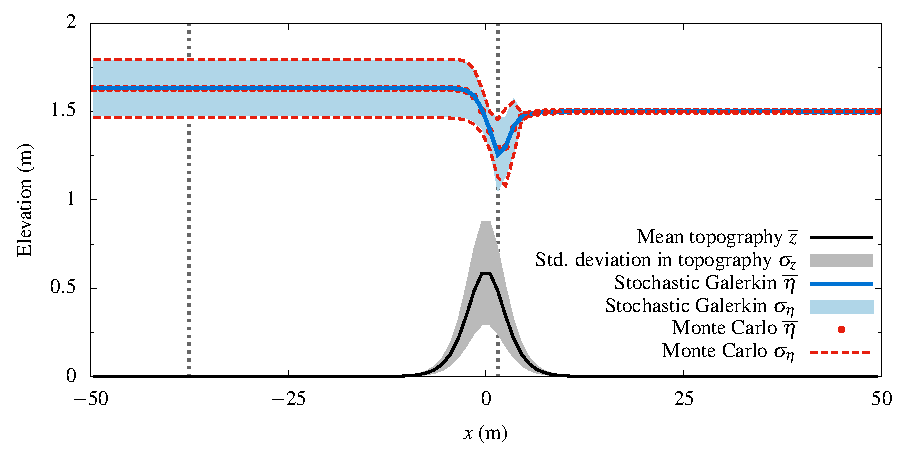
\includegraphics{fig-criticalSteadyState-flow.pdf}
    \caption{Solutions of steady state critical flow over an uncertain hump at $t = \SI{500}{\second}$, comparing stochastic Galerkin and Monte Carlo solutions of (a) water elevation and (b) discharge.
    Standard deviations are plotted using a secondary $y$-axis.
    Vertical lines at $x = \SI{-37.5}{\meter}$ and $x = \SI{1.5}{\meter}$ mark the positions of samples whose distributions are shown in figure~\ref{fig:criticalSteadyState-pdf}.}
    \label{fig:criticalSteadyState-flow}
\end{figure}

For a given flow variable $u = h$ or $u = q$, the probability density function $f(u)$ can be calculated for a given element $i$ and time level $n$,
\begin{subequations}
\begin{align}
        f(u) = \sum_{k=1}^K \Mag{ \sum_{p=0}^P u_{i,p}^{(n)} \frac{\dee \Phi_p}{\dee \xi}(\randomroot_k)}^{-1} W(\randomroot_k)
%
\intertext{where $\randomroot_k$, $k=1, \ldots, K$ are the real roots of the polynomial}
%
        u - \sum_{p=0}^P u_{i,p}^{(n)} \Phi_p(\xi) = 0
\end{align}
\end{subequations}
which can be calculated numerically for a given value of $u$.

\begin{figure}
    \centering
    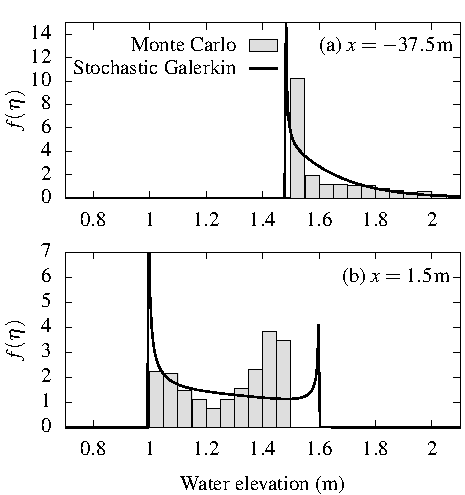
\includegraphics{fig-criticalSteadyState-pdf.pdf}
    \caption{Probability distributions of water elevation at (a) $x = \SI{-37.5}{\meter}$ and (b) $x = \SI{1.5}{\meter}$ for steady state critical flow over an uncertain hump at $t = \SI{500}{\second}$.}
    \label{fig:criticalSteadyState-pdf}
\end{figure}